
\subsubsection{Tendon Constraints}
When modelling tendon length with the constant curvature assumption, one can either assume the tendons are infinitely constrained or finitely constrained. Infinitely constrained tendons result in simpler expressions while finitely constrained tendons are more accurate to feasible implementations \cite{10.3389/frobt.2020.630245}. 


\begin{figure}[h]
    \centering
    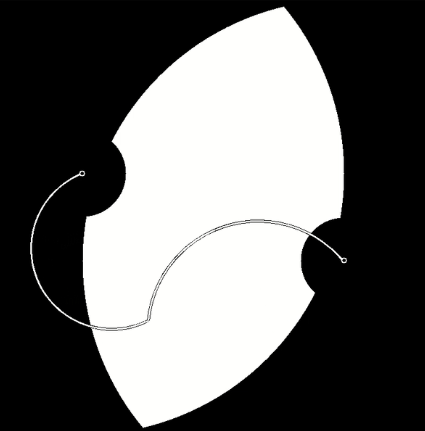
\includegraphics[width=0.4\textwidth]{images/digital_model.png}
    \caption{Digital implementation of baseline model}
    \label{fig:digital_model}
\end{figure}


\subsection{Open Loop Hardware Validation}
In order to compare controllers they must be implemented on the robot. A supervised learning-based controller is unable to provide test results on collected data as the controller is an agent in the system that must be able to affect future data points. As such, testing each model involves running the test trajectories on the physical robot with the controller in the loop as shown in Figure \ref{fig:controller_test}. 

\begin{figure}[h]
    \centering
    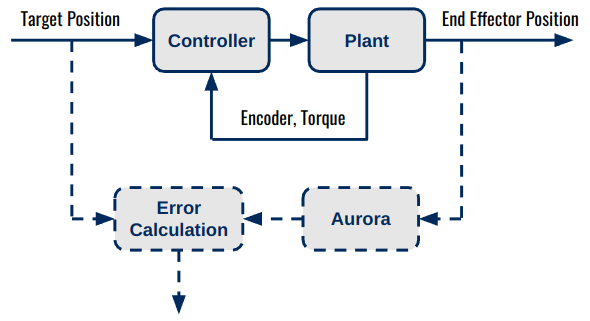
\includegraphics[width=0.7\textwidth]{images/test_control_loop.png}
    \caption{Open loop controller test configuration}
    \label{fig:controller_test}
\end{figure}


\begin{table}[h]
    \centering
    \caption{Continuum robot model comparison}
    \begin{tabular}{l|c|c}
        \textbf{Modelling Method} & \textbf{Accuracy} & \textbf{Complexity} \\
        \hline
        Constant Curvature / Euler Beam Theory & Low & Low \\
        Variable Curvature / Cosserat Rod Theory & High & High \\
        Infinitely Constrained Tendon & Medium & Low \\
        Finitely Constrained Tendon & High & Medium \\
        Data-Driven Approaches & Medium & Medium \\
        Deep Learning Approaches & High & Medium \\
    \end{tabular}   
    \label{tab:model_comparison}
\end{table}